\chapter{Teoria}
\label{ch:teoria}
\begin{it}
	Tähän kohtaan kirjoittaa teoriaa mitä tarvitaan työn toteutuksen ymmärtämisen kannalta. Kaikki työssä tarvittava teoria kuvataan tämän otsikon alla.

	Tämän lukemalla lukija ymmärtää:
	\begin{itemize}
		\item Mikä on standardin ja sähköaseman relaatio ja kuinka ne liittyvät toisiinsa?
		\item Mikä on IEC standardi ja työn kannalta sen tärkeimmät piirtteet.
		\item Kuinka viestien tilaus tapahtuu standardin mukaan?
		\item Kuinka standardi määrittää viestien rakenteen ja parameterit?
		\item Mikä on MMS-protokolla ja kuinka mallinnus standardin objekteista tehdään sille?
	\end{itemize}
\end{it}

Tässä osiossa lukijaa perehdytetään työn kannalta tärkeään teoriaan. Teoriaosuuden kokonaan lukemalla lukija ymmärtää mitä IEC 61850 -standardi tarkoittaa sähköasemien kannalta ja mitä kaikkea se määrittää. Kuinka standardi määrittää tilattavat viestit ja mitä malleja ja palveluita niihin liittyy. Viestien malli ja toiminta on tärkeä ymmärtää työssä toteutetun ohjelman toiminnan kannalta. Työn lopullisessa toteutuksessa viestit prosessoitiin ja julkaistiin jonopalvelimelle myöhempää käyttöä varten. Teorian lopussa lukija perehdytetään jonopalvelimen toteukseen liityvään teoriaan. Myöskin tämän osuuden teoria on tärkeä ymmärtää ohjelman sisäisen toiminnan kannalta.

\section{IEC 61850 -standardi}

Sähköasemilla nykypäivänä käytössä olevilla älykkäillä elektronisilla laitteilla (engl. IED) toteutetaan aseman kontrollointi ja suojaus. Aseman suojauksen lisäksi siihen kuuluu myös asemalta lähtevät sähkölinjat. Jotta suojaus ja ohjaus olisi mahdollista täytyy aseman eri laitteiden kommunikoida verkon yli keskenään ja erilliselle kontrolliasemalle \cite[s.~1]{Brunner2008}. Maailmanlaajuisesti määritetty IEC 61850 -standardi määrittä yhteiset säännöt eri valmistajien laitteiden välille kuinka kommunikointi toteutetaan \cite[s.~10]{IEC61850-7-1}. Ilman yhteisiä sääntöjä jokainen valmistaja olisi vapaa toteuttamaan omat säännöt ja protokollat. Seurauksena olisi, että laitteet eivät olisi keskenään yhteensopivia eri valmistajien välillä. Standardin on tarkoitus poistaa tämä ja määrittää yhteiset pelisäännöt kommunikoinnin toteuttamiseen aseman kommunikointiin liittyen eri laitteiden välillä \cite[s.~1]{Kaneda2008}.

Tärkeä osa standardia on sähköaseman systeemin abstrahointi mallien kautta. Standardi määrittää kuinka abstraktit mallit määritellään aseman oikeista laiteista. Näitä malleja sitten käytetään IED-laitteiden konfiguroinin ja tiedonvälityksen määrittämisessä. Abstraktimallien ansiosta standardi on myös pohjana tulevaisuuden muutoksille. Uusien tekniikoiden ilmaantuessa, voidaan standardin abstraktimallit mallintaa erilliselle tekniikalle, joka mahdollistaa sen \cite[s.~2]{Brunner2008}.

\subsection{Standardin historia}
\begin{it}
	Kirjoita tähän standardin historiaa ja kuinka se muodostui. Pohdi kuitenkin ensin onko tämä lukijan kannalta tärkeää ja tarvittavaa tietoa.
\end{it}

\subsection{Standardin eri osat}

\begin{it}
	Kirjoita tähän aseman funktioiden, fyysisen laitteiden ja loogisten noodien suhteesta toisiinsa. Kuva myös piirrä ja mallia ja tietoa tähän ota \cite[s.~19]{IEC61850-1}
\end{it}
	
IEC 61850 -standardi on todella laaja kokonaisuus. Tämän takia se on pilkottu erillisiin dokumentteihin, josta jokainen käsittelee tiettyä asiaa. Historian saatossa standardiin on lisätty uusia dokumentteja laajentamaan standardia \cite{IEC61850series, New-documents-by-IEC-TC-57}. Tämän työn kirjoitushetkellä standardiin kuului lisäki paljon muitakin dokumentteja, esimerkiksi uusiin mallinnuksiin muille tekniikoille ja vesivoimalaitoksien mallintamiseen liittyviä dokumentteja. Laajuudesta huolimatta standardin voi esittää 10:llä eri pääkohdalla ja näiden alakohdilla. Taulukossa \ref{tab:iec61850-dokumentin-osat} on esitetty standardin pääkohdan dokumentit ja niiden alkuperäiset englanninkieliset otsikot \cite[s.~2]{Mackiewicz2006} \cite{IEC61850series}. Kuvassa \ref{fig:iec61850-osat-ja-relaatiot} on myös esitetty standardin eri osat ja niiden väliset relaatiot.

\begin{table}[ht!]
	\caption{IEC 61850 -standardin pääkohtien ja niiden alakohtien dokumentit.}
	\label{tab:iec61850-dokumentin-osat}
	\begin{tabular}{l | l}
		\hline
		\textbf{Osa} & \textbf{Otsikko englanniksi} \\
		\hline \hline
		1 & Introduction and overview \\
		2 & Glossary \\
		3 & General requirements \\
		4 & System and project management \\
		5 & \parbox[t]{13cm}{Communication requirements for functions and device models} \\
		6 & \parbox[t]{13cm}{Configuration description language for communication in power utility \par automation systems related to IEDs} \\
		7-1 & \parbox[t]{13cm}{Basic communication structure - Principles and models} \\
		7-2 & \parbox[t]{13cm}{Basic information and communication structure - Abstract communication service interface (ACSI)} \\
		7-3 & \parbox[t]{13cm}{Basic communication structure - Common data classes} \\
		7-4 & \parbox[t]{13cm}{Basic communication structure - Compatible logical node classes and data object classes} \\
		8-1 & \parbox[t]{13cm}{Specific communication service mapping (SCSM) - \par  Mappings to MMS (ISO 9506-1 and ISO 9506-2) and to ISO/IEC 8802-3} \\
		9-2 & \parbox[t]{13cm}{Specific communication service mapping (SCSM) - \par  Sampled values over ISO/IEC 8802-3} \\
		9-3 & \parbox[t]{13cm}{Precision time protocol profile for power utility automation} \\
		10 & Conformance testing \\
		\hline
	\end{tabular}
\end{table}

Standardin ensimmäiset osat 1--5 kattavat yleistä kuvaa standardista ja sen vaatimuksista. Osiossa 6 käsitellään IED-laitteiden konfigurointiin käytetty XML (engl. Extensible Markup Language) -pohjainen kieli \cite[s.~7--8]{IEC61850-6}. Tämä osuus ei ole tämän työn kannalta tärkeä ja sitä ei sen tarkemmin käsitellä. Osat 7.1--7.4 käsittelevät standardin abstraktia mallia ja kuinka se rakentuu. Tämä lyhennetään standardissa ACSI (engl. Abstract Communication Service Interface), ja samaa lyhennettä käytetään tässä työssä \cite[s.~72]{IEC61850-7-1}. Osissa 8--9 ja niiden alakohdissa käsitellään abstraktimallien mallintamista erillisille protokollille, jolloin malleista tulee kyseisestä tekniikasta riippuvaisia. Abstrakteja malleja ja niiden mallintamista tekniikalle käsitellään teoriassa tuonnempana. Osa 10 käsittelee testausmenetelmiä, joilla voidaan varmistaa standardin määritysten noudattaminen. Tämä osuus ei myöskään ole tämän työn kannalta tärkeä ja sitä ei teoriassa sen takia käsitellä. \cite[s.~15]{IEC61850-7-1}

\begin{figure}
	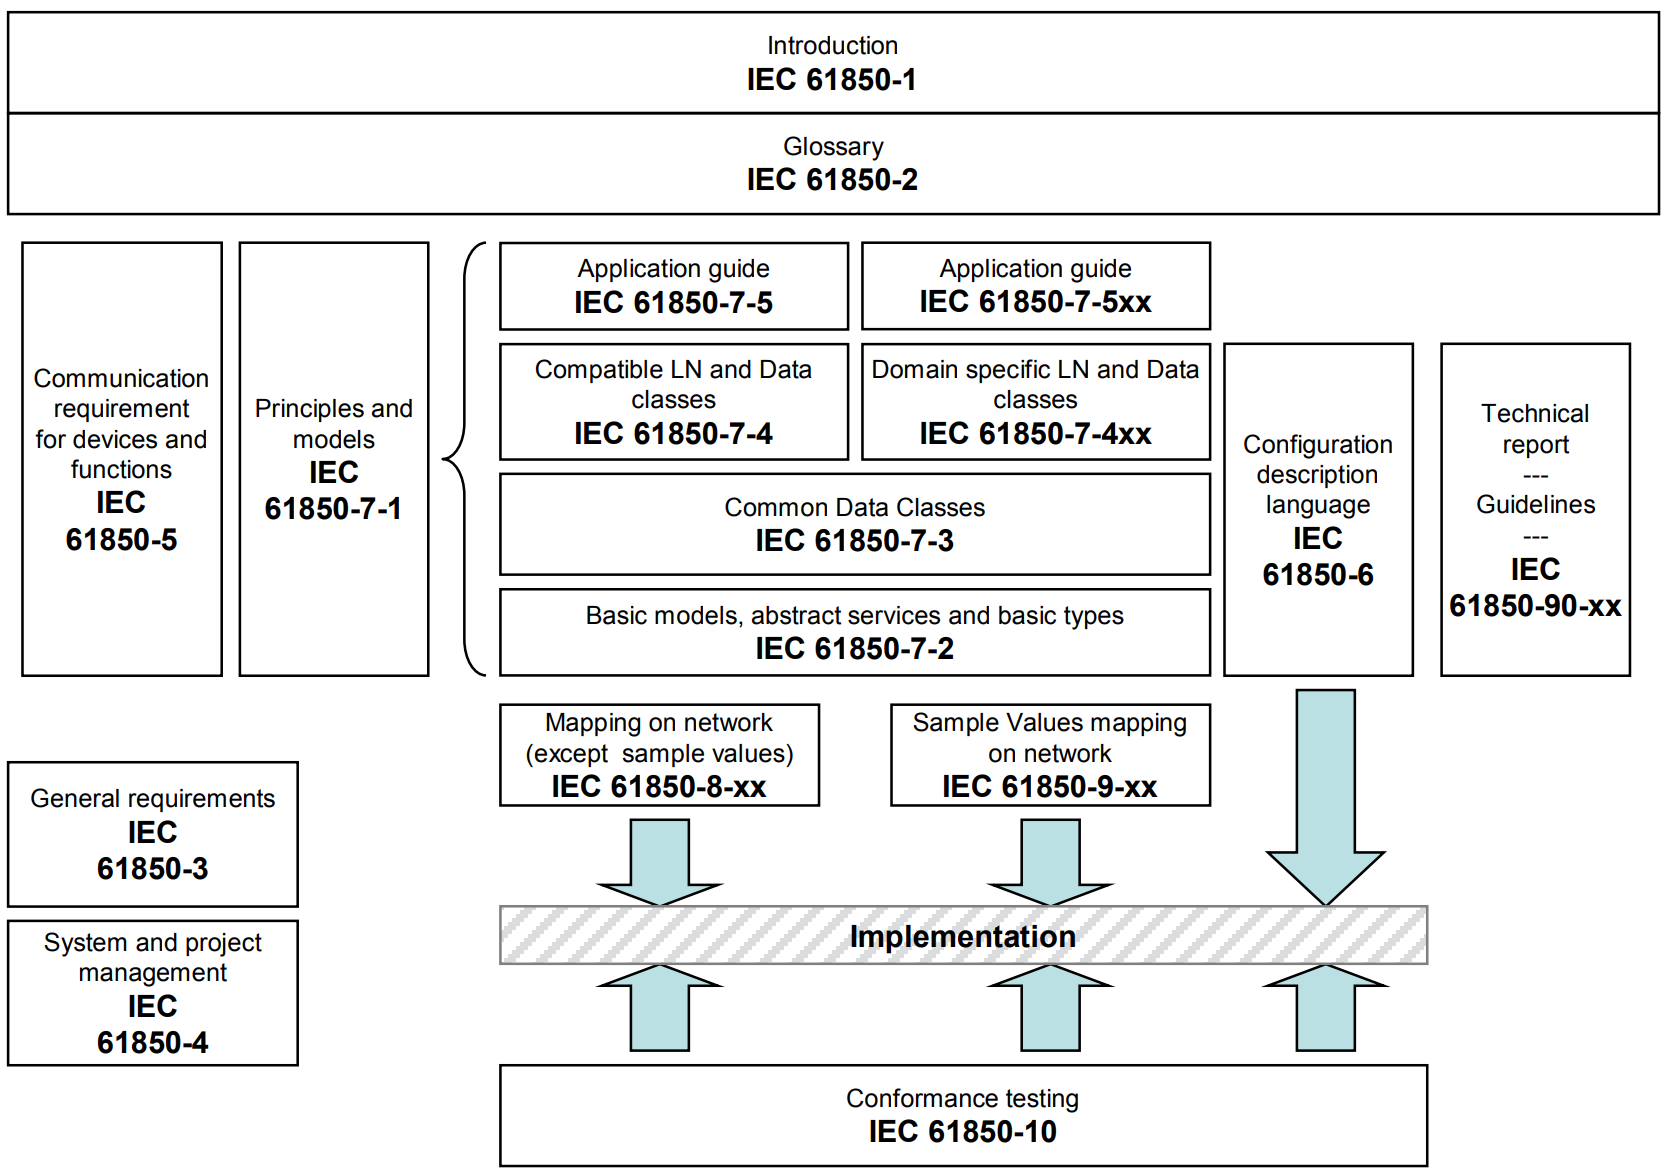
\includegraphics[width=1\textwidth]{pictures/iec-61850-series-and-relations.png}
	\caption{IEC 61850 -standardin osat ja niiden väliset relaatiot \cite[s.~14]{IEC61850-7-1}.}
	\label{fig:iec61850-osat-ja-relaatiot}
\end{figure}

\subsection{Standardin määrittämä abstraktimalli}
\begin{it}
	Kirjoita tähän mitä standardin IEC 61850-7-2 osuudessa määritellään abstraktoimalla fyysisiä laitteita ja palveluita rajapinnoiksi ja olioiksi. Käsittelee standardin Abstract communication service interface (ACSI).

	Piirrä tähän itse esimerkkikuva kuinka standardi mallintaa fyysisen laitteeen loogisiksi laitteiksi. Ota mallia standarin 7-1 kuvasta sivulla 17.

	Kirjoita tähän siitä miten 7-4 osassa on esitetty luokkia ja kuinka ne liittyy 7-3 osan luokkiin. Kuinka näistä muodostetaan instansseja ja mistä arvot tulevat. Tämän jälkeen voisi selittää kuinka polku dataan muodostuu. Tämä voi varmaan olla omana otsikkonaan.
	
	Kirjoita että loogisen noodin data objektit ja attribuutit voidaan kategorisoida 5 eri ryhmään:
	\begin{itemize}
		\item yleinen loogisen noodin informaatio,
		\item tila informaatio,
		\item asetukset, 
		\item mitatut arvot ja
		\item ohjaus \cite[s.~25]{IEC61850-1}.
	\end{itemize}
\end{it}

IEC 61850 -standardin lähtökohtana on pilkkoa koko sähköaseman systeemin funktionaalisuudet pieniksi yksilöiksi. Pilkotut yksilöt abstraktoidaan ja pidetään sopivan kokoisina, jotta ne voidaan konfiguroida esitettäväksi erillisellä IED-laiteella. Esimerkkinä pilkkomisesta voi olla sähköaseman korkean jännitelinjan katkaisija (engl. circuit breaker). Yksi katkaisija vastaisi yhtä pilkottua yksilöä, jonka IED voisi esittää. Näitä pilkottuja yksilöitä kutsutaan standardissa nimellä looginen noodi (engl. logical node ja lyhennetään LN). Loogiset noodit siis mallinetaan jostakin systeemin käsiteellisestä osasta. Loogisia noodeja käytetään rakentamaan looginen laite (engl. logic device, lyhennetään LD). Looginen laite on aseman ohjausyksikkö ja jokin fyysisen laitteen osa, joka toteuttaa loogisten noodien ohjauksen yhtäaikaa. Toisin sanoen loogista laitetta käytetään loogisten noodien yhteiseen ohjaukseen. Looginen laite siis vastaa aseman fyysistä laitetta, joka on kytketty aseman verkkoon ja sillä on IP-osoite. Yksi aseman fyysinen laite voi hoitaa monen loogisen laitteen funktionaalisuuden. Kuvassa X on esitetty standardin eri mallien hierarkia.

\begin{it}
	Sijoita kuva standardin malleista ja niiden relaatioista tähän. Mallia ota ja viite tänne \cite[s.~2]{Camachi2017} \cite[s.~24]{IEC61850-1}
\end{it}

Tässä vaiheessa on hyvä mainita, että standardi pyrkii esittämään aseman toiminnallisuutta hierarkialla ja oliopohjaisesti. Oliopohjaisesti siten, että  standardi määrittää luokkia erilaisille loogisille noodeille. Esimerkiksi katkaisijalle on määritelty luokka nimeltä XCBR (circuit braker). Kun aseman toiminnallisuutta esitetään konfiguraatiossa ja IED-laitteella, luokia instanssioidaan tarpeen mukaan. Standardi määrittää todella paljon erilaisia valmiita luokkia erilaisille loogisille laitteille valmiina käytettäväksi. Standardi myös määrittää laajenoksien mahdollisuudet luokkia käyttäen. Kaikki määritetyt luokat loogisille noodeille voi löytää standardin osasta 7-4. 

Standarissa looginen noodi koostuu data objekteista (engl. data object, lyhennetään DO) ja data objekti monesta data attribuutista (engl. data attribute, lyhennetään DA). Data objekti on tapa koostaa yhteen samaan asiaan liittyvät data attribuutit. Data attribuutit ovat laitteen konfiguroitavia ja luettavia datapisteitä. Data attribuutit kuvaavat fyysisen laitteen tilaa ja mittausarvoja. Esimerkiksi mitattua jännitettä tai katkaisimen tilaa (kiinni tai auki). Kaikki kyseiselle luokalle määritetyt data objektit ja data attribuutit standardi määrittää luokkien määrityksissä dokumentilla 7-3 ja 7-4.

Kaikki edellä mainitut elementit siis muodostavat fyysisestä sähköasemasta hierarkisen olipohjaisen mallin. Hierarkiassa elementit menevät seuraavassa järjestyksessä: logical device (LD) $\rightarrow$ logical node (LN) $\rightarrow$ data object (DO) $\rightarrow$ data attribute (DA).

IEC 61850 -standardin määrittämät konseptit ja abstraktimallit voidaan käyttää myös mallintamaan:
\begin{itemize}
	\item vesivoimalaitos,
	\item sähköasemien välistä kommunikointia,
	\item informaation välitys hajautetun automaation välillä,
	\item informaation välitys sähköaseman ja ohjauskeskuksen välillä,
	\item informaation välitys mittaukseen,
	\item tilan monitorointia ja diagnosointia, ja
	\item informaation välitys konfigurointiin tarkoitetulle tekniikalle \cite[s.~11]{IEC61850-7-1}.
\end{itemize}


\subsection{Standardin luokkien rakenne}
\begin{it}
	Kirjoita tähän kuinka standardin loogiset noodit rakentuvat. Kerro mitä common data classes sisältää ja kuinka ne määrittää data monessa paikassa käytetyt data attribuutit. Tämän jälkeen kuinka loogisen noodin luokat rakennetaan käyttämällä CDC määrityksiä \cite[s.~26]{IEC61850-1}. Ota tähän myös kuvia taulukosta ja rakenna esimerkkinä yksi looginen noodi niitä käyttäen. Tätä samaa mallia voi myöhemmin käyttää määrittämään kuinka referensssipolut luokkien nimillä rakentuu.
\end{it}

\subsection{Viestiblokin konfigurointi ja tilaus}
\begin{it}
	Kirjoita tähän IEC 61850 -standardin määrittästä abstraktista raportointimallista. Tätä raportointi mekanismia tullaan käyttämään raporttien tilauksessa ja sen konfigurointi täytyy ymmärtää toteuttettavan ohjelmiston kannalta.
\end{it}

\subsection{Viestin rakenne}
\begin{it}
	Kirjoita tähän standardin määritämästä viestin rakenteesta ja mitä tietoa se sisältää. Kerro myös sen vaihtoehtoisista kentistä.
\end{it}

\section{Abstraktimallin sovitus MMS-protokollaan}
\begin{it}
	Kirjoita kuinka ylempi ACSI sovitetaan MMS-protokollan palveluiksi ja tietotyypeiksi standardin IEC 61850-8-1 osuuden mukaan. Tähän myös miten raportointi toimii MMS-protokollan päällä.
\end{it}

\subsection{MMS-protokolla}
\begin{it}
	Selitä lyhyesti mikä on MMS-protokolla ja vähän sen tietotyypeistä. Tämän tarkoitus on pohjustaa tulevaa IEC 61850 abstraktien olioiden (ACSI) sovitusta tämän protokollan päälle.
\end{it}

\section{Advanced Message Queuing Protocol}
\begin{it}
	Kirjoita tähän AMQP määrittävästä standardista, mikä sen tarkoitus on ja mihin sitä voidaan käyttää.
\end{it}

\subsection{Viestien välitysmekanismit}
\begin{it}
	Mitä mekanismeja AMQP tarjoaa viestien välittämiseen osapuolille. Näitä on jono, reititys suoraan osapuolien välillä ja viestin julkaisu ja tilaaminen.
\end{it}

\subsection{Tilaus ja julkaisu -mallin osat}
\begin{it}
	Kirjoita tähän AMQP tarjoamista viestien julkaisu ja tilaus -mallin osista osapuolten kesken. Kerro mitä eri osat tekevät ja mikä niiden tehtävä viestien välittämisessä on. Englanniksi osia ovat esim. exchange, queue, publisher ja consumer.
\end{it}